\documentclass[11pt,twoside]{article}

% Do NOT use ANY packages other than asp2023. 
\usepackage{asp2023}
\usepackage{comment}

\aspSuppressVolSlug
\resetcounters

\bibliographystyle{asp2021}

\markboth{Femia et al.}{Event Classification of Terrestrial Gamma-ray Flashes}

\begin{document}

\title{Machine-Learning-Based Event Classification \\ of Terrestrial Gamma-ray Flashes \\ with a Segmented Scintillator Detector}

\author{
A.~Femia,$^{1}$ 
N.~Parmiggiani,$^{1}$ 
A.~Bulgarelli,$^{1}$ 
V.~Fioretti,$^{1}$ 
L.~Castaldini,$^{1}$ 
M.~Maniscalco,$^{1,5}$ 
G.~Panebianco,$^{1}$ 
A.~Di~Piano,$^{1}$ 
R.~Falco,$^{1}$ 
G.~Mustafa,$^{1}$ 
A.~Rizzo,$^{2}$ 
A.~De~Rosa,$^{1}$ 
E.~Virgilli,$^{1}$ 
C.~Labanti,$^{1}$ 
M.~Marisaldi,$^{3}$ 
F.~Calzolari,$^{4}$ 
A.Marinoni,$^{4}$
C.Pittori $^{6}$
}


\affil{$^{1}$INAF/OAS Bologna, Via P. Gobetti 93/3, 40129 Bologna, Italy;
\email{antonio.femia@inaf.it}}

\affil{$^2$INAF - Osservatorio Astrofisico di Catania, Via Santa Sofia 78, Catania, 95123, Italy}

\affil{$^3$Birkeland Centre for Space Science, Department of Physics and Technology, University of Bergen, Norway}

\affil{$^4$CNR-ISAC, Via P. Gobetti 101, I-40129 Bologna, Italy}

\affil{$^5$Università degli Studi di Padova, Via VII Febbraio , 2, 35122, Padova, Italy}

\affil{$^6$INAF/OAR Roma, Via di Frascati 33, I-00078 Monte Porzio Catone, Italy}

% This section is for ADS Processing.  There must be one line per author. paperauthor has 9 arguments.
\paperauthor{A.~Femia}{antonio.femia@inaf.it}{0000-0001-5978-4784}
{INAF/OAS Bologna}{}
{Bologna}{BO}{40129}{Italy}

\paperauthor{N.~Parmiggiani}{nicolo.parmiggiani@inaf.it}{0000-0002-4535-5329}
{INAF/OAS Bologna}{}
{Bologna}{BO}{40129}{Italy}

\paperauthor{A.~Bulgarelli}{andrea.bulgarelli@inaf.it}{0000-0001-6347-0649}
{INAF/OAS Bologna}{}
{Bologna}{BO}{40129}{Italy}

\paperauthor{V.~Fioretti}{valentina.fioretti@inaf.it}{0000-0002-6082-5384}
{INAF/OAS Bologna}{}
{Bologna}{BO}{40129}{Italy}

\paperauthor{L.~Castaldini}{luca.castaldini@inaf.it}{0009-0000-5501-4328}
{INAF/OAS Bologna}{}
{Bologna}{BO}{40129}{Italy}

\paperauthor{M.~Maniscalco}{mattia.maniscalco@inaf.it}{0009-0004-0219-1282}
{INAF/OAS Bologna}{Univerity of Padova}
{Bologna}{BO}{40129}{Italy}

\paperauthor{G.~Panebianco}{gabriele.panebianco@inaf.it}{0000-0002-3410-8613}
{INAF/OAS Bologna}{}
{Bologna}{BO}{40129}{Italy}

\paperauthor{A.~Di~Piano}{ambra.dipiano@inaf.it}{0000-0002-9894-7491}
{INAF/OAS Bologna}{}
{Bologna}{BO}{40129}{Italy}

\paperauthor{R.~Falco}{luca.castaldini@inaf.it}{0009-0004-1676-7596}
{INAF/OAS Bologna}{}
{Bologna}{BO}{40129}{Italy}

\paperauthor{G.~Mustafa}{luca.castaldini@inaf.it}{0009-0005-1088-9119}
{University of Bologna}{Department of Computer Science and Engineering}
{Bologna}{BO}{40126}{Italy}

\paperauthor{A.~Rizzo}{alessandro.rizzo@inaf.it}{0009-0003-4341-2988}
{INAF/OA Catania}{}
{Catania}{CT}{95123}{Italy}

\paperauthor{E.~Virgilli}{enrico.virgilli@inaf.it}{0000-0003-2279-9119}
{INAF/OAS Bologna}{}
{Bologna}{BO}{40129}{Italy}

\paperauthor{C.~Labanti}{enrico.virgilli@inaf.it}{0000-0002-5086-3619}
{INAF/OAS Bologna}{}
{Bologna}{BO}{40129}{Italy}

\paperauthor{M.~Marisaldi}{martino.marisaldi@inaf.it}{0000-0002-4000-3789}
{Birkeland Centre for Space Science}{Department of Physics and Technology}
{Bergen}{NO}{5007}{Norwey}

\paperauthor{F.P.~Calzolari}{francescopiero.calzolari@cnr.it}{0000-0003-4535-9626} {CNR-ISAC}
{Bologa}{BO}{-40129}{Italy}

\paperauthor{C.~Pittori}{carlotta.pittori@inaf.it}{0000-0001-6661-9779} {INAF/OAR Roma}{}
{Roma}{RM}{I-00078}{Italy}



\begin{abstract}
The detection of Terrestrial Gamma-ray Flashes (TGFs) from CubeSat-class spacecraft presents significant challenges due to their sub-millisecond duration, the presence of backgrounds, and stringent onboard computational and power constraints. This work investigates a machine-learning-based approach for charged-particle background rejection in a compact, segmented gamma-ray detector designed for CubeSat-class missions. The detector consists of $500$ GAGG scintillator crystals, providing three-dimensional spatial and energy-deposition information. Monte Carlo simulations are performed using MEGAlib/Geant4 to model the response of the segmented GAGG detector to TGF photons and charged particles. A dedicated machine-learning classifier is developed to discriminate TGF photons from charged-particle backgrounds. %Quantization and pruning techniques are applied to reduce computational and memory requirements for embedded deployment.
Preliminary results, obtained without modelling atmospheric attenuation of TGF photons, demonstrate the potential of combining detector segmentation and machine-learning classification for future space-based TGF observations.
\end{abstract}



\section{Introduction}
Terrestrial Gamma-ray Flashes (TGFs) are sub-millisecond bursts of atmospheric gamma rays associated with thunderstorms. Their observation provides valuable insights into high-energy particle acceleration processes in the Earth's atmosphere, and TGFs have been extensively studied through satellite observations. Observations by Fermi-GBM, AGILE-MCAL, and ASIM have demonstrated that TGF photon energies can extend to several tens of MeV, providing valuable information on the acceleration processes occurring within thunderstorms \citep{Lindanger2021,Marisaldi2010,Ursi2019}.

Space-based TGF observations are challenged by the extremely short duration, which can lead to detector dead time and pulse pile-up, affecting their measured temporal and spectral properties \citep{Briggs2010}. Electromagnetic radiation and charged particles interact with scintillators through different physical processes, potentially producing distinguishable energy-deposition patterns. Segmented scintillator architectures enable the measurement of energy deposits in individual detector elements, providing information on hit multiplicity, energy sharing, and the three-dimensional spatial distribution of deposited energy \citep{SalehNatur2026}. These observables can be exploited by machine-learning algorithms to support background discrimination.

As part of the GammaSky project \citep{Castaldini2026}, this study investigates the response of a segmented scintillator detector to photons in the 10 keV--40 MeV energy range. The detector consists of 500 GAGG (Gadolinium Aluminum Gallium Garnet, $\mathrm{Gd_3Al_2Ga_3O_{12}}$) scintillator crystals, each measuring $1 \times 1 \times 0.8\ \mathrm{cm^3}$.
The crystals are separated by $0.2\ \mathrm{cm}$ gaps
along the $Z$-axis, and the detector has a volume filling factor of 50\% (see the left panel of
Figure~\ref{fig:geometry_occupancy}).  The high density ($6.63\ \mathrm{g/cm^3}$) and effective atomic number of GAGG provide high gamma-ray interaction probability within a compact volume, while the inter-crystal gaps house the readout cables and associated electronics.

%As part of the GammaSky project \citep{Castaldini2026}, this study investigates the ability of a segmented scintillator detector to discriminate TGF photons from charged-particle backgrounds using Monte Carlo simulations and machine-learning-based event classification.


%The study also addresses the computational constraints associated with onboard processing, aiming to develop an efficient classification strategy suitable for future CubeSat-class high-energy instruments.

\section{Methodology}
\label{sec:methodology}

All simulations were performed using MEGAlib (Medium Energy Gamma-ray Astronomy Library), an open-source framework based on Geant4 for modelling particle transport and interactions in gamma-ray detectors \citep{Zoglauer2006}. % over the keV–GeV energy range.
 %MEGAlib relies on Geant4 for modelling particle transport
%and interactions with matter.

The simulated charged-particle background \citep{Cumani2019, Gallego2026} includes primary and secondary electrons ($e^-$), primary and secondary positrons ($e^+$), primary alpha particles
(${}^{4}\mathrm{He}^{2+}$), and primary and secondary
protons ($p^+$). Secondary protons are further distinguished into upward-going particles (originating from Earth) and downward-going particles (arriving from the sky). Background simulations were based on the integral particle flux expected in low Earth orbit (LEO), considering an observation time of $1000\,\mathrm{s}$ at an orbital altitude of $550\,\mathrm{km}$. The energy spectra for each charged-particle background component are depicted in the right panel of Figure \ref{fig:geometry_occupancy}. 
The incident TGF photon spectrum was modeled, neglecting the atmospheric attenuation,  using an RREA (Relativistic Runaway Electron Avalanche)-like exponentially cut-off power law:

\begin{equation}
\frac{dN_\gamma}{dE}
\propto E^{-1}
\exp\left(-\frac{E}{7.3\,\mathrm{MeV}}\right),
\label{eq:tgf_spectrum}
\end{equation}

\noindent
with photon energies spanning from $10\,\mathrm{keV}$ to $40\,\mathrm{MeV}$.

\begin{figure}[!ht]
    \centering

    \begin{minipage}[t]{0.35\textwidth}
        \centering
        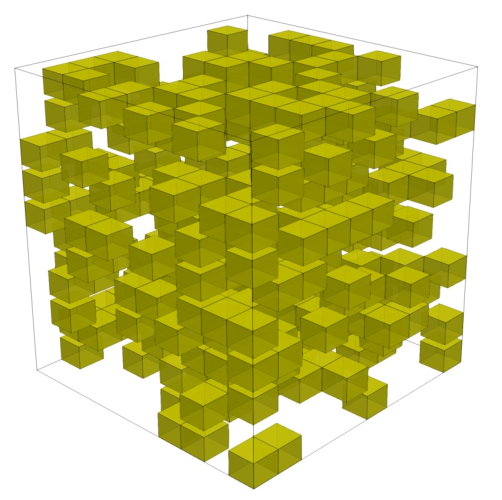
\includegraphics[width=\linewidth]{3dView.pdf}
    \end{minipage}
    \hfill
    \begin{minipage}[t]{0.55\textwidth}
        \centering
        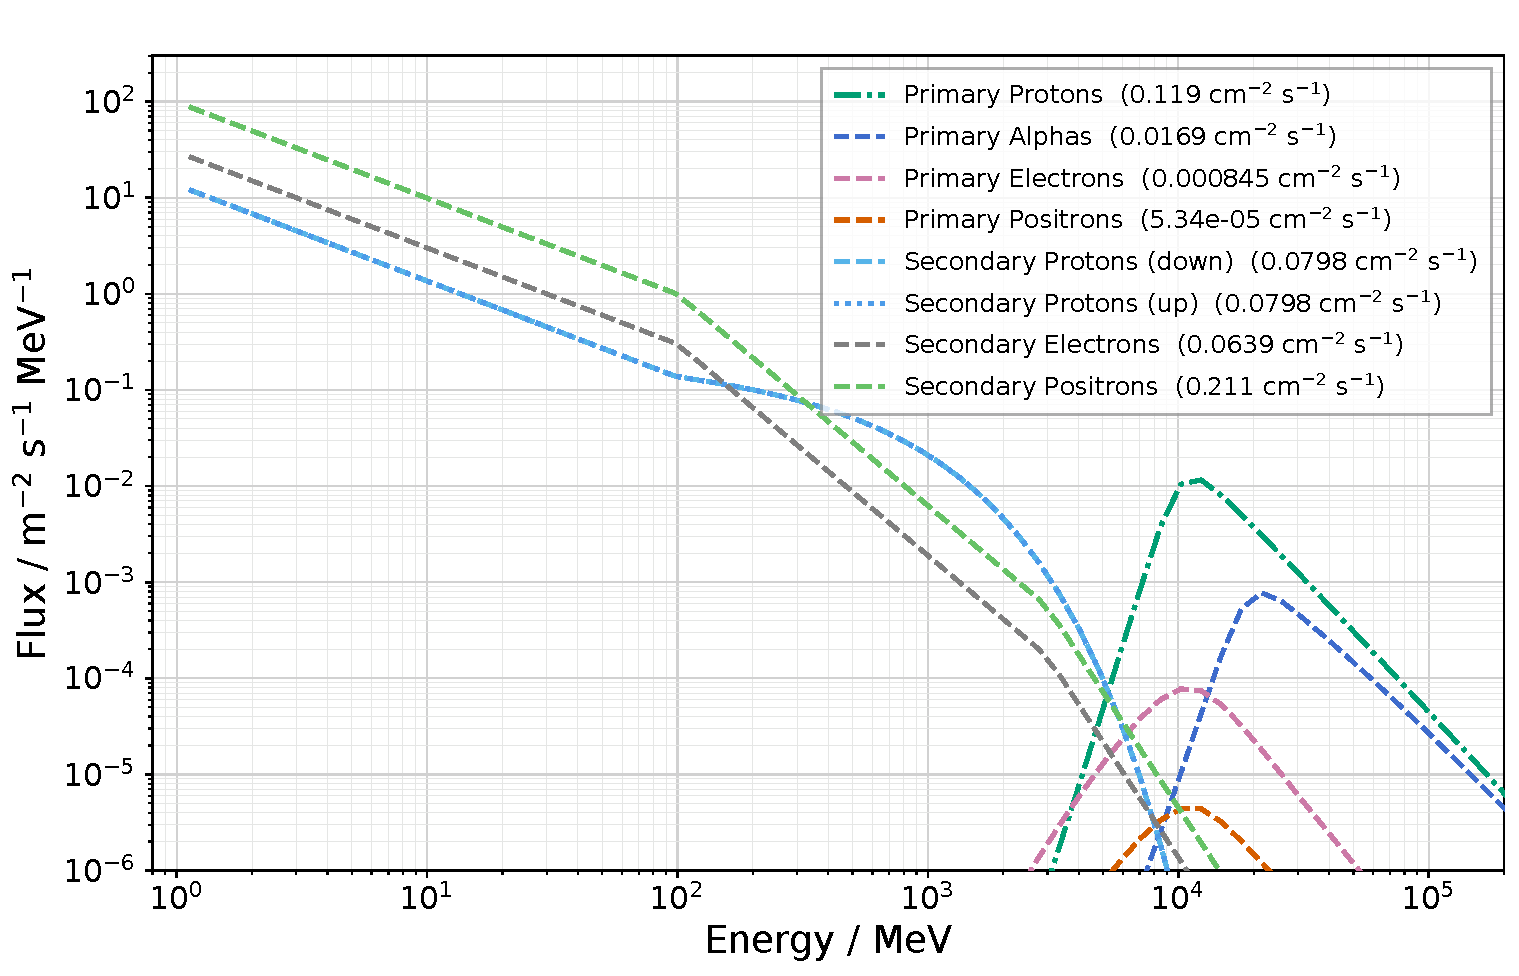
\includegraphics[width=\linewidth]{charged_background_spectra.pdf}
    \end{minipage}

    \caption{Detector geometry and energy spectrum.
    \textit{Left:} Three-dimensional view of the segmented
    GAGG detector geometry.
    \textit{Right:} Differential energy spectra, for charged-particle backgrounds, assuming a solar modulation potential
    of 650 MV.}

    \label{fig:geometry_occupancy}
\end{figure}

\begin{comment}
    
\begin{figure}[!ht]
    \centering

    \begin{minipage}[t]{0.49\textwidth}
        \centering
        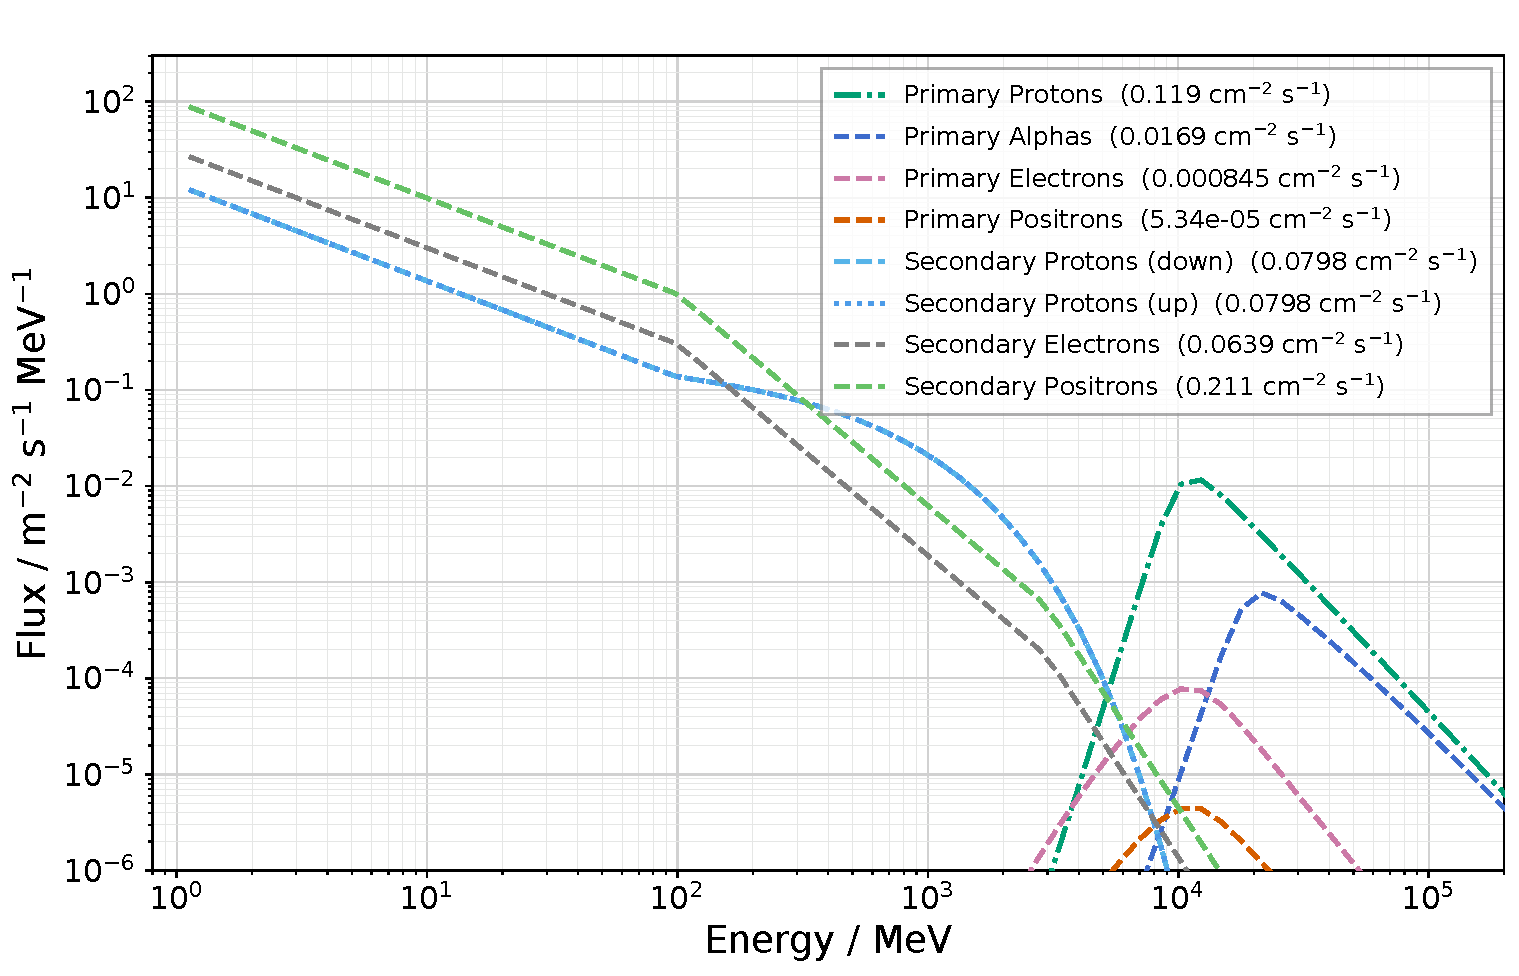
\includegraphics[width=\linewidth]{charged_background_spectra.pdf}
    \end{minipage}
    \hfill
    \begin{minipage}[t]{0.49\textwidth}
        \centering
        \includegraphics[width=\linewidth]{background_rate_hz_charged.pdf}
    \end{minipage}

    \caption{Charged-particle background at an orbital altitude of 550 km.
    \textit{Left:} Differential energy spectra assuming a solar modulation potential
    of 650 MV.
    \textit{Right:} Event rates.}

    \label{fig:charged_background}
\end{figure}
\end{comment}

\begin{figure}[!ht]
    % \caption{Simulated detector response to TGF photons and
charged-particle backgrounds.
\textit{Left:} Mean number of lit GAGG pixels and pixel
multiplicity distributions for each particle component.
\textit{Right:} Event rates and hit rates for the different
charged-particle background components. %, with total rates
%of 82.2 Hz and 507.1 Hz, respectively.

    \label{fig:background_characterization}
\end{figure}

\section{Classifier Architecture}
\label{sec:classifier_architecture}

The classifier is based on a fully connected feed-forward neural network, taking 49 standardised physics-inspired features as input. The architecture consists of two hidden dense layers with 128 and 64 neurons, respectively, employing ReLU activation functions and dropout regularisation (p = 0.1). Batch normalisation is applied after the first dense layer to improve training stability. The output layer contains two neurons for binary classification between TGF photons and charged-particle background. To exploit the spatial information provided by the segmented
detector, only events activating at least three pixels
($n_{\mathrm{pixels}} \geq 3$) were selected for machine-learning classification. %This requirement retains 54.83\% of charged-particle background events and 5.23\% of TGF events. 
%Since low-energy TGF photons generally activate fewer than three pixels, this selection mainly excludes low-energy interactions. 
%A total of 49 physics-inspired features were extracted from the simulated detector response and organized into five categories.
\begin{comment}
\begin{itemize}
    \item Energy deposition and multiplicity: pixel multiplicity, total deposited energy, statistical moments, energy percentiles, and dispersion measures.

    \item Energy sharing and concentration:
    energy entropy, Gini coefficient, active-pixel
    fractions, and energy concentration.

    \item Spatial geometry and topology:
    energy-weighted center of mass, radius of gyration,
    spatial covariance eigenvalues, linearity, planarity,
    sphericity, asymmetry, and spatial extent.

    \item Hit statistics:
    total hit count, mean hits per active pixel,
    and energy--hit correlations.

    \item Morphological complexity:
    fractal dimension, connectivity, maximum path
    length, branching structure, and skeleton length.
\end{itemize}
\end{comment}

%These features characterise the energetic and geometrical signatures of particle interactions, providing complementary information for distinguishing TGF photons from charged-particle backgrounds.

\section{Results}
\label{sec:results}
The left panel of Figure \ref{fig:background_classification} shows the pixel-hit multiplicity distributions obtained for TGF photons and charged-particle background events. TGF photons exhibit a mean pixel multiplicity of 1.25, with most events activating a single pixel. Charged-particle backgrounds show higher mean multiplicities, ranging from 3.37--3.40 for secondary protons to 28.60 for primary electrons, with primary alpha particles and protons averaging 16.53 and 10.35 pixels, respectively.

The classifier achieves a receiver operating characteristic area under the curve (ROC AUC) of 0.981 on the selected test dataset, with an overall classification accuracy of 92.3\%. A TGF recall of 97.8\% is obtained, corresponding to 6,725 correctly identified signal events out of 6,876, with a signal precision of 82.6\%. Simultaneously, 89.6\% of charged-particle background events are correctly rejected (see the right panel of Figure \ref{fig:background_classification}). %As a representative example, the results for electrons are presented in Figure \ref{fig:background_characterization}. In the 10--30 MeV range, the classifier achieves a signal recall of 88.1\%, an electron-background rejection of 93.4\%, and a macro-averaged F1 score of 0.879. For energies above 30 MeV, electron-background rejection increases to 98.9\%, while retaining 90.0\% of TGF events.
Overall, these results highlight the potential of combining energy-deposition statistics and spatial topology for charged-particle background rejection. %, particularly in the high-energy TGF regime.



\begin{figure}[!ht]
    \centering

    \begin{minipage}[t]{0.6\textwidth}
        \centering
        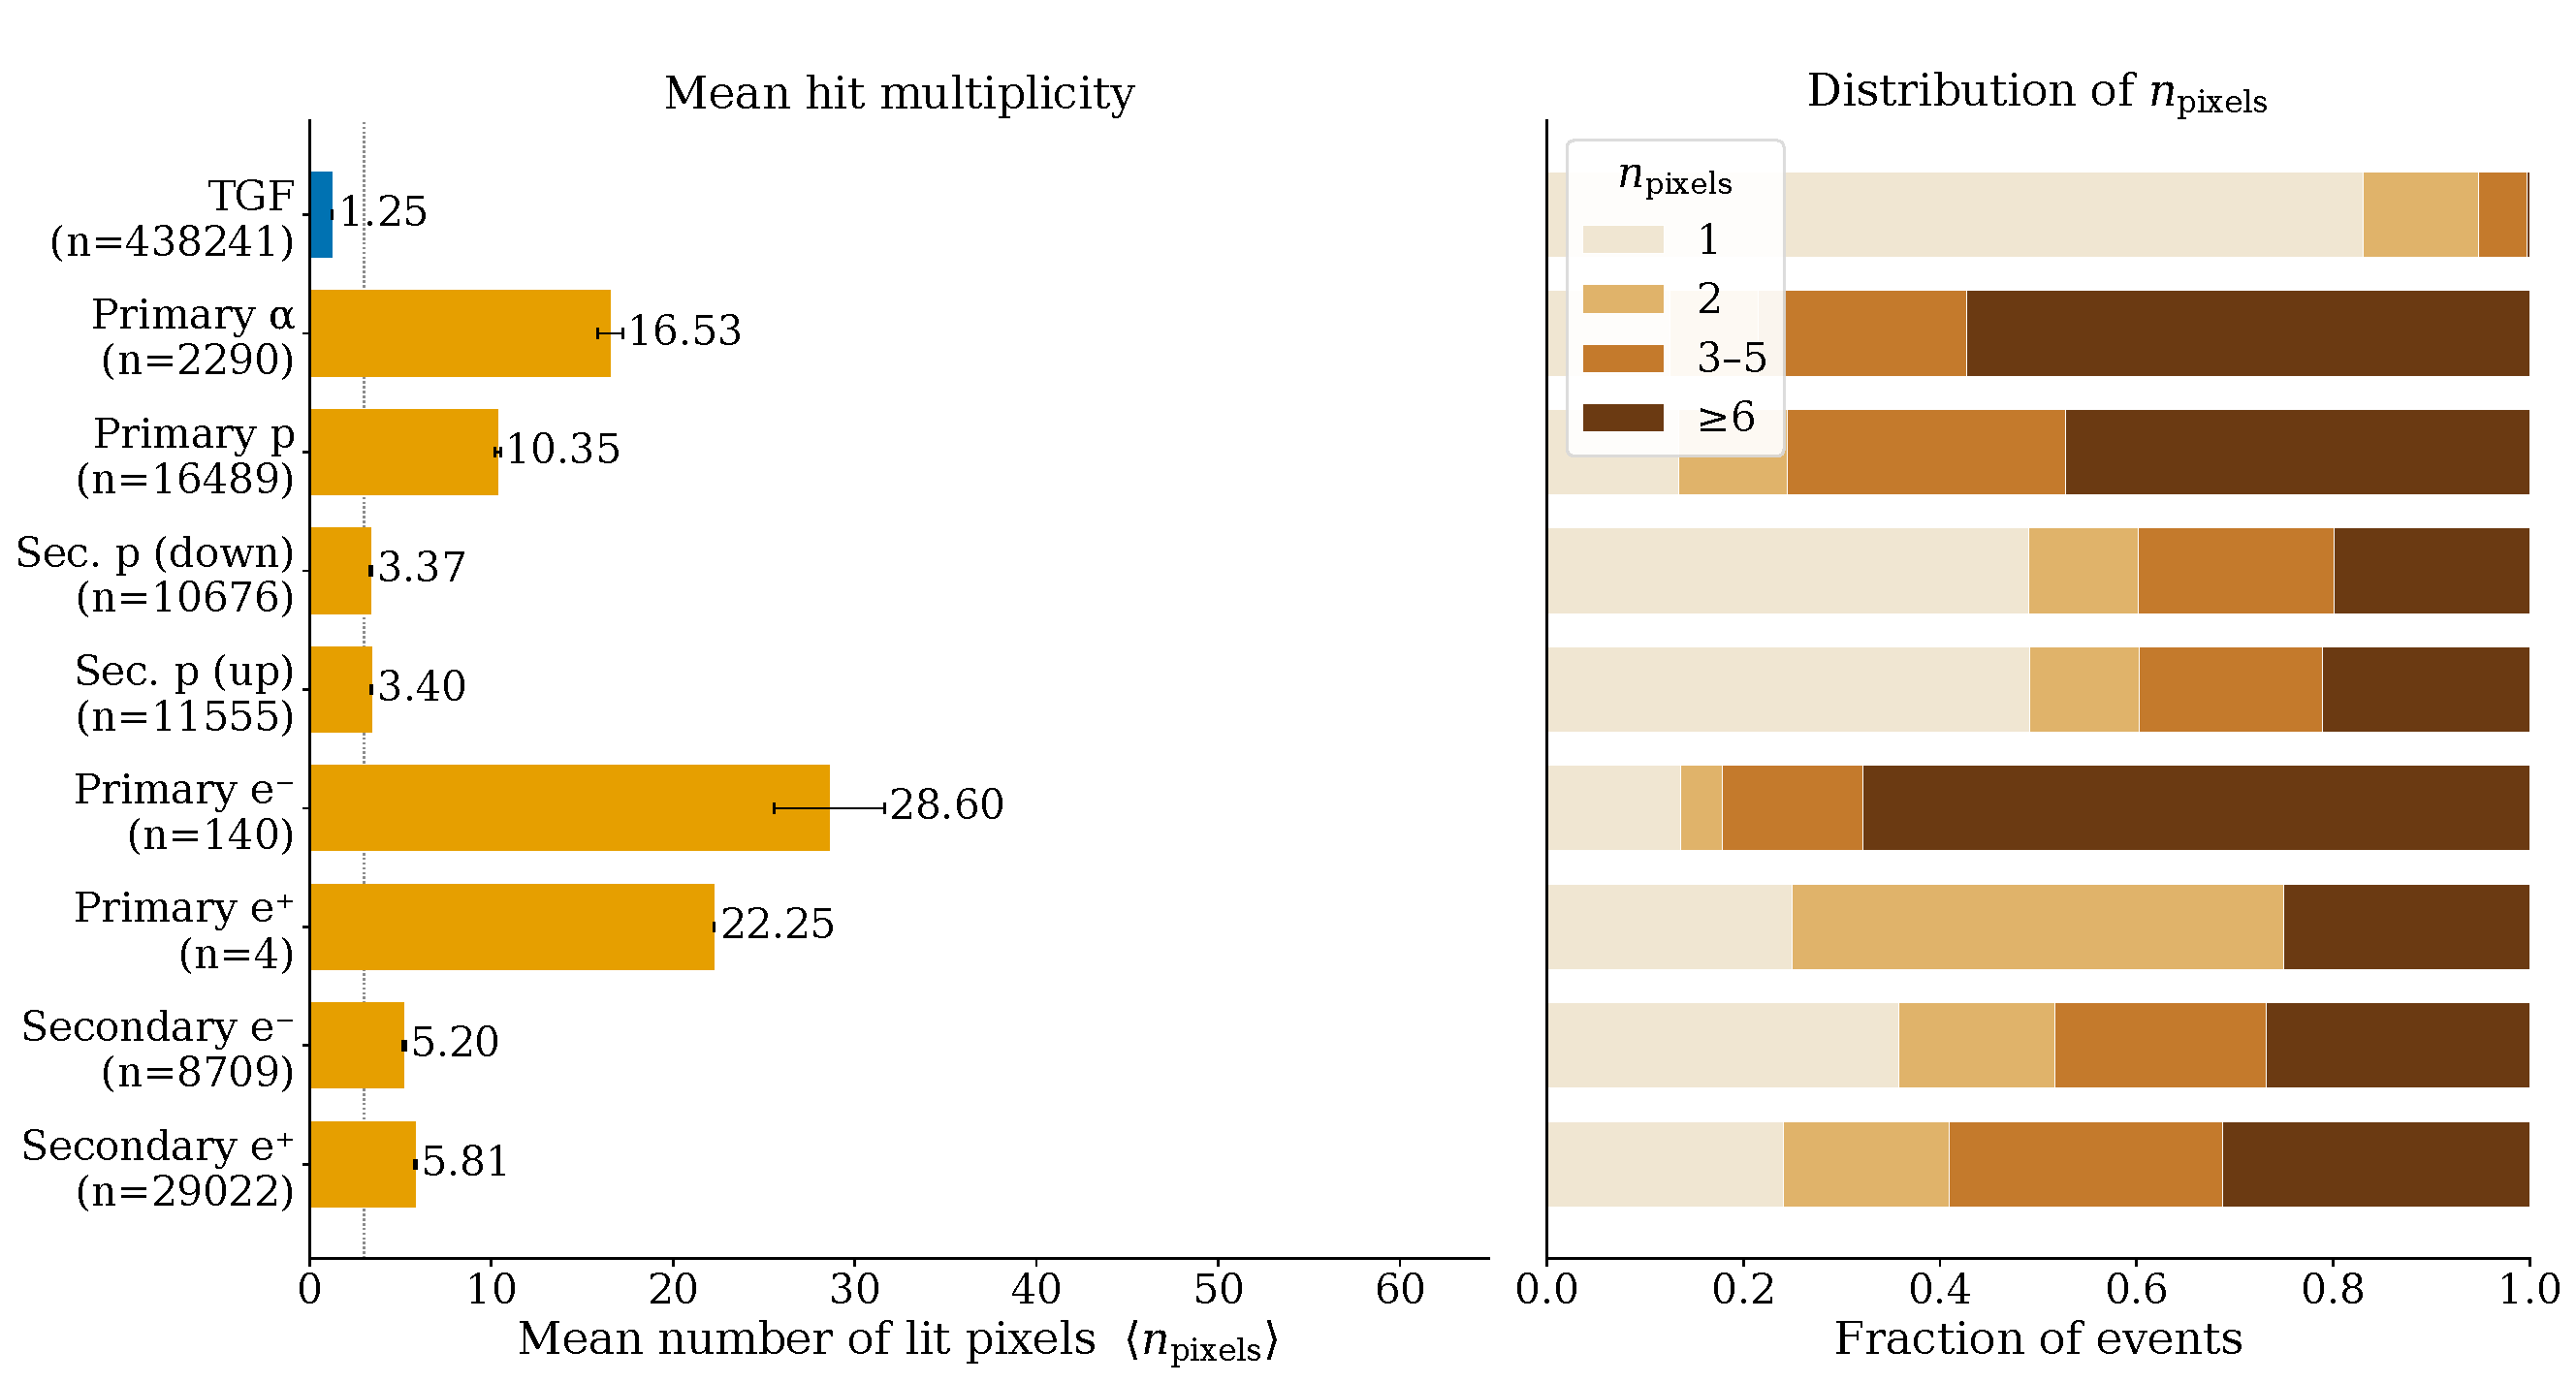
\includegraphics[width=\linewidth]{mean_n_voxels_by_component.pdf}
    \end{minipage}
    \hfill
    \begin{minipage}[t]{0.35\textwidth}
        \centering
        \includegraphics[width=\linewidth]{tab_confusion_matrix.pdf}
    \end{minipage}

    \caption{Hit distributions and machine learning classification performance.
    \textit{Left:} Mean number of lit pixels and pixel
    multiplicity distributions for TGF photons and
    charged-particle background components.
    \textit{Right:} Confusion matrix for events with
    $n_{\mathrm{pixels}}\geq 3$.}

    \label{fig:background_classification}
\end{figure}



\section{Conclusions}
In this work, a segmented GAGG scintillator detector was proposed for TGF observations. The high density and effective atomic number of GAGG enable efficient gamma-ray absorption, while the segmented design provides a mass-efficient architecture suitable for CubeSat-class missions. Furthermore, the modular architecture offers improved fault tolerance, as failures of scintillator channels do not necessarily compromise the entire instrument, allowing continued operation. A fully connected neural network was developed to discriminate TGF photons from charged-particle backgrounds, achieving a ROC AUC of 0.981, a TGF recall of 97.8\%, and a charged-particle background rejection of 89.6\% on the preselected test dataset. These findings highlight the potential of combining segmented scintillator detectors with machine learning for future CubeSat-class TGF observations and motivate further optimisation and onboard validation.


\bibliography{P207}  % For BibTex

% if we have space left, we might add a conference photograph here. Leave commented for now.
% \bookpartphoto[width=1.0\textwidth]{foobar.eps}{FooBar Photo (Photo: Any Photographer)}

\end{document}
